% !TeX root = ../../Book3.tex
% 纲要标题：### 15.5* Cheeger–Gromoll 分裂
% 纲要位置：几何学计划纲要.md，第 2737 行。
% 正文状态：初稿；尚未正式审核。

% 纲要内容开始
% 
% * 直线与两侧 Busemann 函数
% * 弱 Laplace 比较与最大值原理
% * Busemann 的调和性和光滑性
% * Bochner 公式与平行单位梯度
% * 整体等距乘积的构造
% 
% ---
% 
% 纲要内容结束

\OptionalSection{Cheeger–Gromoll 分裂}{g3:sec:1505}

一条测地线可以无限延长，却未必在远处仍然最短。如果它的任意有限段都最短，两端同时通向无穷远，就能产生两个相互制约的距离极限。第八章已经用它们构造了弱次调和函数；现在借助强最大值原理、椭圆正则性与 Bochner 公式，可以把这个极限变成一个平行单位梯度。本节证明 Cheeger--Gromoll 分裂定理\footnote{Jeff Cheeger（1943--），美国数学家，研究黎曼几何与几何分析，在曲率界、流形结构和奇点的定量研究方面作出贡献。 Detlef Gromoll（1938--2008），德国数学家，长期在美国工作，研究整体微分几何、非负曲率流形与测地线，参与建立灵魂定理。}：连通完备无边界流形若具有非负 Ricci 曲率并含有测地直线，便有一个整体的等距 \(\mathbb R\) 因子。

\ProseParagraphBreak

距离比较负责找到候选坐标，局部分析负责使它光滑，完备性则使坐标方向的流存在任意长时间。最后一项还不能省去：局部的平行场只有在能够全时流动、并且来自全局实值函数时，才会给出这里需要的全局乘积。以下继续使用 \(\Delta=-\operatorname{div}\nabla\)，以及沿射线增加的 Busemann 符号。

\subsection{直线与两侧 Busemann 函数}
\label{g3:subsec:1505:01}
回顾\cref{g3:def:busemann-function}，单位速测地射线 \(\eta:[0,\infty)\to M\) 满足 \(d(\eta(s),\eta(t))=|s-t|\)。测地直线则有整个实轴作参数域，并对任意 \(s,t\in\mathbb R\) 满足同一距离等式。两个条件都包含最短性；单是速度恒为一、参数域无界，还不足以称为射线或直线。

\begin{lemma}\label{g3:lem:line-two-busemann-limits}
	设 \((M,g)\) 为连通、完备、光滑、无边界的黎曼流形，\(\gamma:\mathbb R\to M\) 为单位速测地直线。对 \(T\ge0\) 令
	\[
		b_{+,T}(x)=T-d(x,\gamma(T)),\qquad
		b_{-,T}(x)=T-d(x,\gamma(-T)).
	\]
	则两者随 \(T\to\infty\) 分别在紧集上一致收敛到 \(1\)-Lipschitz 函数 \(b_+,b_-\)，且
	\begin{equation}\label{g3:eq:splitting-busemann-sum}
		b_++b_-\le0,\qquad
		b_+(\gamma(s))=s,\qquad b_-(\gamma(s))=-s
		\quad(s\in\mathbb R).
	\end{equation}
\end{lemma}
\begin{proof}
	这是\cref{g3:prop:busemann-basic}用于两个方向的情形，下面恢复极限中会用到的估计。对任一射线 \(\eta\)，当 \(T\ge S\) 时，三角不等式给出
	\[
		d(x,\eta(T))\le d(x,\eta(S))+T-S,
	\]
	所以 \(T-d(x,\eta(T))\) 单调增加。它又处在 \([-d(x,\eta(0)),d(x,\eta(0))]\) 内，因而有有限极限。每个近似函数均为 \(1\)-Lipschitz，极限保持这一性质。若 \(K\) 紧，取其有限 \(\varepsilon\)-网；先使网点处的近似误差小于 \(\varepsilon\)，再用两次 Lipschitz 估计，就使整个 \(K\) 上的误差小于 \(3\varepsilon\)。这证明局部一致收敛。

	直线的两端相距 \(2T\)，故
	\[
		d(x,\gamma(T))+d(x,\gamma(-T))\ge2T.
	\]
	取极限得到和不大于零。对固定 \(s\in\mathbb R\)，只要 \(T>|s|\)，就有
	\(b_{+,T}(\gamma(s))=T-(T-s)=s\)、
	\(b_{-,T}(\gamma(s))=T-(T+s)=-s\)。因此它们的和在整条直线上等于零。
\end{proof}

两侧函数的和已经在内部点达到全局最大值。若再知道它是弱次调和的，强最大值原理就会把直线上的等号传播到整个流形。这里不需要在远处给函数加边界值；直线本身已经提供了一个达到最大值的位置。

\subsection{弱 Laplace 比较与最大值原理}
\label{g3:subsec:1505:02}
距离函数在割迹上不一定光滑，Busemann 极限也最初只有 Lipschitz 正则性。因此比较不等式须与紧支测试函数配对，再令远端趋于无穷。这样的极限只涉及固定紧集上的函数值。

\begin{proposition}\label{g3:prop:line-busemann-opposites}
	设 \((M^n,g)\) 连通、完备、光滑、无边界，\(n\ge2\)，\(\operatorname{Ric}\ge0\)，并含有单位速测地直线 \(\gamma\)。则\(b_\pm(x)=\lim_{T\to\infty}(T-d(x,\gamma(\pm T)))\) 属于 \(C^0(M)\cap H^1_{\mathrm{loc}}(M)\)，并满足
	\[
		\Delta b_+\le0,\qquad \Delta b_-\le0
		\quad\text{于分布意义下},\qquad b_++b_-=0.
	\]
\end{proposition}
\begin{proof}
	先核对一阶弱正则性。在一个相对紧坐标盒中，局部 Lipschitz 函数沿每条坐标直线都是 Lipschitz 的一元函数，因而绝对连续，其导数几乎处处存在且有一致界。逐条直线分部积分，再用 Fubini，可得各坐标弱偏导属于 \(L^\infty\)。度量和密度在较小坐标盒上有界且非退化，所以函数属于该盒上的 \(H^1\)。有限个局部片覆盖任一紧集，证明 \(b_\pm\in H^1_{\mathrm{loc}}\)。连续性由 Lipschitz 性给出。

	现在恢复\cref{g3:prop:busemann-weak-laplacian}的分布极限。固定非负 \(\phi\in C_c^\infty(M)\)，令 \(K=\operatorname{supp}\phi\)，并取 \(C\) 使 \(d(x,\gamma(0))\le C\) 对所有 \(x\in K\) 成立。当 \(T>C\) 时，
	\[
		r_{\pm,T}(x):=d(x,\gamma(\pm T))\ge T-C>0
		\quad(x\in K).
	\]
	\cref{g3:thm:distributional-laplacian-comparison}的 \(k=0\) 情形给出
	\(\Delta r_{\pm,T}\ge-(n-1)/r_{\pm,T}\)。又因 \(\phi\) 紧支，散度定理给出 \(\int_M\Delta\phi\,\mu_g=0\)，于是
	\begin{equation}\label{g3:eq:busemann-distribution-limit}
		\int_M b_{\pm,T}\Delta\phi\,\mu_g
		\le\frac{n-1}{T-C}\int_M\phi\,\mu_g.
	\end{equation}
	在 \(K\) 上的一致收敛保证左侧趋于 \(\int b_\pm\Delta\phi\,\mu_g\)，右侧趋于零。因此 \(\Delta b_\pm\le0\)。对 \(H^1_{\mathrm{loc}}\) 函数，坐标弱分部积分还把该式写成
	\[
		\int_M\langle\mathrm db_\pm,\mathrm d\phi\rangle\,\mu_g\le0.
	\]
	这恰是\cref{g3:thm:weak-subharmonic-strong-maximum}所用的弱次调和不等式。

	令 \(u=b_++b_-\)。它连续且属于 \(H^1_{\mathrm{loc}}\)，满足 \(\Delta u\le0\)，并由式\eqref{g3:eq:splitting-busemann-sum}知 \(u\le0\)、\(u(\gamma(0))=0\)。\(M\) 连通且无边界，所以该强最大值原理给出 \(u\equiv0\)。
\end{proof}

这一推导保留了割迹在分布比较中的贡献。即使极限函数随后变得光滑，近似距离的比较仍须使用第七章已经证明的分布版本；逐点略过割迹不能提供式\eqref{g3:eq:busemann-distribution-limit}。

\subsection{Busemann 的调和性和光滑性}
\label{g3:subsec:1505:03}
两个非正分布的和为零，使它们分别为零。由此得到光滑性以后，还需确定梯度的长度。Lipschitz 估计只给出上界；从任意点出发、把最短线的另一端推向无穷远，则提供达到这个上界的方向。

\begin{proposition}\label{g3:prop:line-busemann-smooth-harmonic}
	设 \((M^n,g)\) 连通、完备、光滑、无边界，\(n\ge2\)、\(\operatorname{Ric}\ge0\)，并含有单位速测地直线 \(\gamma:\mathbb R\to M\)。则两侧 Busemann 函数 \(b_\pm(x)=\lim_{T\to\infty}(T-d(x,\gamma(\pm T)))\) 都是光滑调和函数。
\end{proposition}
\begin{proof}
	由前一命题，\(b_-=-b_+\)。对每个非负测试函数 \(\phi\)，有
	\[
		\langle\Delta b_+,\phi\rangle\le0,
		\qquad
		-\langle\Delta b_+,\phi\rangle
		=\langle\Delta b_-,\phi\rangle\le0,
	\]
	所以这两个数都为零。任意实测试函数 \(\psi\) 都能写成两个非负光滑紧支函数之差：取在 \(\operatorname{supp}\psi\) 附近等于一的非负截断 \(\chi\)，再取 \(A\ge\|\psi\|_\infty\)，则
	\(\psi=(\psi+A\chi)-A\chi\)。故 \(\Delta b_+=0\) 对全部测试函数成立，\(b_-\) 同样如此。

	前一命题已核对 \(H^1_{\mathrm{loc}}\) 正则性，故\cref{g3:prop:weak-harmonic-smoothing}适用，给出光滑调和代表。该代表与原连续函数几乎处处相等，实际上处处相等：若某点的差不为零，连续性会使差在一个开邻域内保持非零，违反几乎处处相等。因此原来的距离极限本身就是光滑调和函数。
\end{proof}

\begin{lemma}\label{g3:lem:busemann-calibrated-ray}
	设 \((M,g)\) 连通、完备、光滑且无边界，\(\eta:[0,\infty)\to M\) 为单位速测地射线，\(b(x)=\lim_{T\to\infty}(T-d(x,\eta(T)))\)。对每个 \(x\in M\)，存在从 \(x\) 出发的单位速测地射线 \(\sigma_x\)，使
	\begin{equation}\label{g3:eq:busemann-calibrated-ray}
		b(\sigma_x(s))=b(x)+s\qquad(s\ge0).
	\end{equation}
	若 \(b\) 在 \(x\) 可微，则 \(|\nabla b(x)|=1\)，且所有满足上述等式的单位初速度都等于 \(\nabla b(x)\)。
\end{lemma}
\begin{proof}
	取 \(T_j\to\infty\)。由\cref{g3:thm:hopf-rinow}，存在从 \(x\) 到 \(\eta(T_j)\) 的单位速最短测地线
	\[
		\sigma_j:[0,\ell_j]\to M,\qquad
		\ell_j=d(x,\eta(T_j))\ge T_j-d(x,\eta(0))\longrightarrow\infty.
	\]
	其初速度属于紧的有限维单位球面 \(S_xM\)。取子列使 \(\dot\sigma_j(0)\to v\)，其中 \(|v|=1\)，并令 \(\sigma_x(s)=\exp_x(sv)\)。完备性使这个表达对全部 \(s\ge0\) 有定义；\cref{g3:thm:geodesic-ivp}的光滑初值依赖说明 \(\sigma_j\) 在每个有限参数区间上收敛到 \(\sigma_x\)。对固定 \(0\le s<t\)，充分大的 \(j\) 有 \(\ell_j>t\)，故
	\[
		d(\sigma_x(s),\sigma_x(t))
		=\lim_jd(\sigma_j(s),\sigma_j(t))=t-s.
	\]
	所以极限确为射线。

	记 \(b_T=T-d(\cdot,\eta(T))\)。最短线的尾段仍最短，故对固定 \(s\) 及充分大的 \(j\)，
	\[
		b_{T_j}(\sigma_j(s))
		=T_j-(\ell_j-s)=b_{T_j}(x)+s.
	\]
	取任意 \(A>s\)，这些点都在紧闭球 \(\overline B(x,A)\) 内。\cref{g3:prop:busemann-basic}的紧集一致收敛，以及 \(\sigma_j(s)\to\sigma_x(s)\)，使等式可取极限，得到式\eqref{g3:eq:busemann-calibrated-ray}。同一个初速度子列对每个固定 \(s\) 都适用，所以所得等式成立于整个半轴。

	若 \(b\) 在 \(x\) 可微，沿这条射线在零点求右导数得
	\[
		1=\mathrm db_x(v)=\langle\nabla b(x),v\rangle.
	\]
	另一方面，\(b\) 的 \(1\)-Lipschitz 性沿任意单位速短测地线求导给出 \(|\nabla b(x)|\le1\)。结合 \(|v|=1\) 与 Cauchy--Schwarz 不等式，必有 \(|\nabla b(x)|=1\)，且等号条件给出 \(v=\nabla b(x)\)。
\end{proof}

把这个引理用于已经光滑的 \(b=b_+\)，得到处处成立的 \(|\nabla b|=1\)。极限射线一旦成为梯度轨道，其初方向就不再依赖先前抽取的子列。这样，从距离极限得到的不只是调和函数，还是一个没有临界点、沿指定方向以单位速度增加的全局坐标候选。

\subsection{Bochner 公式与平行单位梯度}
\label{g3:subsec:1505:04}
单位梯度尚可随位置旋转；这种变化由 Hessian 测量。非负 Ricci 曲率与调和性一起，使 Bochner 公式中的两个非负量同时消失。这里使用的是逐点恒等式，无须对整个非紧流形积分。

\begin{proposition}\label{g3:prop:line-busemann-parallel-gradient}
	设 \((M^n,g)\) 连通、完备、光滑、无边界，\(n\ge2\)、\(\operatorname{Ric}\ge0\)，并含有单位速测地直线 \(\gamma\)。令 \(b(x)=\lim_{T\to\infty}(T-d(x,\gamma(T)))\) 为其正向 Busemann 函数，标量 Laplace 取 \(\Delta=-\operatorname{div}\operatorname{grad}\)，则
	\[
		\Delta b=0,\qquad |\nabla b|=1,\qquad
		\operatorname{Hess}b=0,
		\qquad \operatorname{Ric}(\nabla b,\nabla b)=0.
	\]
	因此 \(X=\nabla b\) 是平行单位向量场，\(\mathcal D=X^\perp=\ker\mathrm db\) 是平行分布；\(b\) 的各水平集都是光滑全测地超曲面。
\end{proposition}
\begin{proof}
	前一小节给出前两式。由\cref{g3:thm:bochner-function}，按本书的非负 Laplace 约定，
	\[
		\frac12\Delta|\nabla b|^2
		=\langle\nabla\Delta b,\nabla b\rangle
		-|\operatorname{Hess}b|^2
		-\operatorname{Ric}(\nabla b,\nabla b).
	\]
	左侧为零，右侧第一项也为零；其余两个被减去的量都非负。因此它们逐点为零。由
	\(\operatorname{Hess}b(Y,Z)=\langle\nabla_YX,Z\rangle\)，得到 \(\nabla X=0\)。

	若 \(Y\) 与 \(X\) 正交，则对任意 \(Z\)，
	\[
		\langle\nabla_ZY,X\rangle
		=Z\langle Y,X\rangle-\langle Y,\nabla_ZX\rangle=0.
	\]
	所以正交分布平行。由于 \(\mathrm db\ne0\)，常秩定理说明水平集为光滑超曲面，其切空间恰为 \(\ker\mathrm db\)。对水平集上的切向量场 \(Y,Z\)，法向第二基本形式为
	\(\langle\nabla_YZ,X\rangle=-\langle Z,\nabla_YX\rangle=0\)，故水平集全测地。
\end{proof}

平坦环面提供一个需要辨明的整体情形：常向量场可以下降为平行单位场，但其对偶一形式在某个闭路上的积分可能非零，因此不是全局实值函数的微分。环面上没有 \(\mathbb R\) 因子；它是紧的，任何两点的距离都受直径约束，也不可能包含测地直线。分裂证明中保留下来的全局函数 \(b\)，正是用来给每条梯度轨道指定唯一的零水平交点。

\subsection{整体等距乘积的构造}
\label{g3:subsec:1505:05}
取 \(N=b^{-1}(0)\)，希望把 \((t,x)\in\mathbb R\times N\) 送到从 \(x\) 沿 \(X=\nabla b\) 流动时间 \(t\) 的点。为了让这个定义产生整体等距同构，须依次核对流的全时存在、每条轨道与 \(N\) 的唯一相交，以及微分怎样保持长度。

\termidx[Cheeger Gromoll fenlie dingli]{Cheeger--Gromoll 分裂定理}
\foreignidx{Cheeger--Gromoll splitting theorem}
\begin{theorem}[Cheeger--Gromoll 分裂定理]\label{g3:thm:cheeger-gromoll-splitting}
	设 \((M^n,g)\) 为连通、完备、光滑、无边界黎曼流形，\(n\ge1\)，且 \(\operatorname{Ric}_M\ge0\)。若存在单位速测地直线 \(\gamma:\mathbb R\to M\)，则存在连通、完备、光滑、无边界的 \((n-1)\) 维黎曼流形 \((N,g_N)\)，满足 \(\operatorname{Ric}_N\ge0\)，以及整体等距同构
	\[
		F:(\mathbb R\times N,\mathrm dt^2+g_N)\longrightarrow(M,g).
	\]
	令 \(b_+(x)=\lim_{T\to\infty}(T-d(x,\gamma(T)))\)，可以取 \(N=b_+^{-1}(0)\)，使 \(b_+(F(t,x))=t\)，且 \(F(t,\gamma(0))=\gamma(t)\)。当 \(n=1\) 时，\(N\) 为一个点。反过来，每个这样的黎曼乘积都含有测地直线。
\end{theorem}
\begin{proof}
	先设 \(n\ge2\)。前面各结果给出全局光滑函数 \(b=b_+\)，其梯度 \(X\) 平行且长度为一。取 \(X\) 的最大局部流 \(\Phi_t\)。若某条积分曲线仅定义到有限正时刻 \(T\)，则对 \(s,t<T\)，有
	\[
		d(\Phi_s(p),\Phi_t(p))\le|s-t|,
	\]
	因为曲线速度为一。因此 \(t\uparrow T\) 时曲线形成 Cauchy 族；度量完备性给出极限点 \(p_T\in M\)。在 \(p_T\) 附近的坐标中，光滑向量场的局部存在唯一性可将这条解越过 \(T\) 延拓，违反最大性。负时间同理，故 \(\Phi_t\) 对全部 \(t\in\mathbb R\) 存在，并且关于 \((t,p)\) 光滑。流的唯一性给出 \(\Phi_{s+t}=\Phi_s\circ\Phi_t\)、\(\Phi_t^{-1}=\Phi_{-t}\)。这里使用的常微分方程结果与\cref{g3:thm:geodesic-ivp}中构造测地流的结果相同。

	沿流求导得到
	\begin{equation}\label{g3:eq:busemann-flow-translation}
		\frac{\mathrm d}{\mathrm dt}b(\Phi_t(p))
		=\mathrm db(X)=|X|^2=1,
		\qquad b(\Phi_t(p))=b(p)+t.
	\end{equation}
	因此 \(N=b^{-1}(0)\) 非空，至少含有 \(\gamma(0)\)，且每条轨道恰在时间 \(-b(p)\) 到达 \(N\)。定义
	\begin{equation}\label{g3:eq:splitting-flow-map}
		F(t,x)=\Phi_t(x),\qquad
		F^{-1}(p)=\bigl(b(p),\Phi_{-b(p)}(p)\bigr).
	\end{equation}
	由式\eqref{g3:eq:busemann-flow-translation}，逆公式中的第二项确实属于 \(N\)。将两个公式相互代入，利用流群律，得到两个恒等映射；两式又都光滑，故 \(F\) 是整体微分同胚。此时尚不预设 \(N\) 连通：映射 \(p\mapsto\Phi_{-b(p)}(p)\) 连续且满射到 \(N\)，而 \(M\) 连通，所以 \(N\) 连通。

	接着验证度量。固定初点处的向量 \(Y,Z\)，把它们沿流推前为 \(Y_t=(\Phi_t)_*Y\)、\(Z_t=(\Phi_t)_*Z\)。例如取初速度为 \(Y\) 的曲线 \(q(s)\)，则 \(Y_t\) 是二参数变分 \(\Phi_t(q(s))\) 的 \(s\) 方向导数。两个参数方向可交换；无挠性与 \(\nabla X=0\) 因而给出
	\[
		\nabla_XY_t=\nabla_{Y_t}X=0,\qquad
		\nabla_XZ_t=0.
	\]
	因此
	\(\frac{\mathrm d}{\mathrm dt}g(Y_t,Z_t)=0\)，说明每个 \(\Phi_t\) 都是等距映射。另一方面，对 \(v\in \mathrm T_xN\)，将式\eqref{g3:eq:busemann-flow-translation}对初点求导，得
	\[
		\mathrm db_{\Phi_t(x)}((\Phi_t)_*v)=\mathrm db_x(v)=0.
	\]
	所以 \((\Phi_t)_*v\) 与 \(X\) 正交。对 \(a,c\in\mathbb R\) 及 \(v,w\in \mathrm T_xN\)，
	\[
		\mathrm dF_{(t,x)}(a,v)=aX_{\Phi_t(x)}+(\Phi_t)_*v,
	\]
	从而
	\[
		g(\mathrm dF(a,v),\mathrm dF(c,w))
		=ac+g_N(v,w).
	\]
	于是 \(F^*g=\mathrm dt^2+g_N\)，所构造的微分同胚确为整体等距同构。

	还须核对 \(N\) 的完备性。它是连续函数 \(b\) 的闭水平集。对 \(x,y\in N\)，任何 \(N\) 中的曲线也是 \(M\) 中的曲线，故 \(d_M(x,y)\le d_N(x,y)\)。反过来，把连接 \(x,y\) 的任意 \(M\) 中曲线用 \(F^{-1}\) 写成 \((t(s),z(s))\)，再投影到 \(N\)，长度不增加，因为
	\[
		|z'(s)|_{g_N}\le\sqrt{|t'(s)|^2+|z'(s)|_{g_N}^2}.
	\]
	取长度下确界得到 \(d_N(x,y)\le d_M(x,y)\)，所以两个距离在 \(N\times N\) 上相等。\(N\) 的内在 Cauchy 列因而在完备的 \(M\) 中收敛；闭性使极限仍在 \(N\)，距离相等又保证内在收敛。因此 \(N\) 完备。它的光滑性、无边界及维数来自 \(\mathrm db\ne0\) 的正则水平集描述。

	在乘积度量中，将 \(N\) 上的向量场沿 \(\mathbb R\) 常值延拓。Koszul 公式给出切向联络等于 \(N\) 的联络，且 \(\nabla\partial_t=0\)；所以切向曲率等于 \(R_N\)，含 \(\partial_t\) 的曲率项为零。对 \(Y\in\mathrm TN\)，在正交标架 \((\partial_t,e_1,\ldots,e_{n-1})\) 中取迹，得到
	\[
		\operatorname{Ric}_M(Y,Y)=\operatorname{Ric}_N(Y,Y)\ge0.
	\]
	沿给定直线，\(b(\gamma(t))=t\)，故
	\(\langle X,\dot\gamma\rangle=1\)。两个向量都是单位向量，因而 \(X|_\gamma=\dot\gamma\)。积分曲线唯一性给出 \(F(t,\gamma(0))=\gamma(t)\)。

	当 \(n=1\) 时可直接处理。直线 \(\gamma\) 的微分处处可逆，所以其像是开集；若 \(\gamma(t_j)\) 在 \(M\) 中收敛，则 \(|t_j|=d(\gamma(0),\gamma(t_j))\) 有界，取子列即知极限仍在其像中。因此像也闭。连通性使 \(\gamma\) 满射，而距离等式保证它单射且等距，于是 \(M\cong\mathbb R\)，取 \(N\) 为一点即可。

	最后，在任意乘积 \(\mathbb R\times N\) 中，曲线 \(t\mapsto(t,x_0)\) 速度为一。连接 \((s,x_0)\) 与 \((t,x_0)\) 的曲线长度至少为其 \(\mathbb R\) 投影的长度，因而至少为 \(|t-s|\)；该曲线自身达到这个下界，所以它是测地直线。
\end{proof}

\begin{figure}[htbp]
	\centering
	% !TeX root = ../Book3.tex
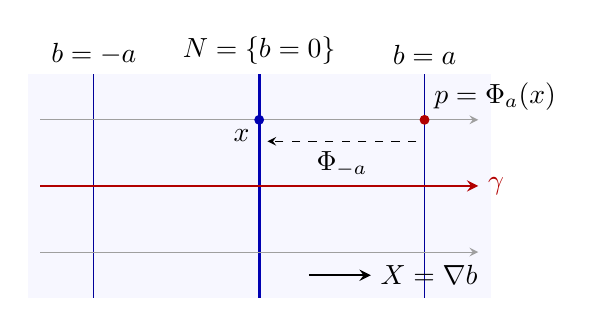
\begin{tikzpicture}[>=stealth,scale=1.05]
	\fill[blue!3] (-2.8,-1.35) rectangle (2.8,1.35);
	\draw[blue!60!black] (-2,-1.35)--(-2,1.35);
	\draw[very thick,blue!70!black] (0,-1.35)--(0,1.35);
	\draw[blue!60!black] (2,-1.35)--(2,1.35);
	\node[above] at (-2,1.35) {\(b=-a\)};
	\node[above] at (0,1.35) {\(N=\{b=0\}\)};
	\node[above] at (2,1.35) {\(b=a\)};
	\draw[->,gray!75] (-2.65,-.8)--(2.65,-.8);
	\draw[->,thick,red!70!black] (-2.65,0)--(2.65,0);
	\node[right,red!70!black] at (2.65,0) {\(\gamma\)};
	\draw[->,gray!75] (-2.65,.8)--(2.65,.8);
	\fill[blue!70!black] (0,.8) circle (1.7pt);
	\fill[red!70!black] (2,.8) circle (1.7pt);
	\node[below left] at (0,.8) {\(x\)};
	\node[above right] at (2,.8) {\(p=\Phi_a(x)\)};
	\draw[->,dashed] (1.9,.54)--(.1,.54);
	\node[below] at (1,.54) {\(\Phi_{-a}\)};
	\draw[->,thick] (.6,-1.08)--(1.35,-1.08);
	\node[right] at (1.35,-1.08) {\(X=\nabla b\)};
\end{tikzpicture}

	\caption[平行梯度流与水平集乘积]{平行梯度流把 \(N=b^{-1}(0)\) 等距地送到各水平集。点 \(p\) 的乘积坐标是 \((b(p),\Phi_{-b(p)}p)\)。图中水平箭头表示流轨道，纵向线表示水平集；它们的平面形状只用于标示相交关系。}
	\label{g3:fig:splitting-flow}
\end{figure}

\begin{example}\label{g3:exm:ray-without-line-paraboloid}
	在 \(\mathbb R^3\) 中取抛物面 \(P=\{z=x^2+y^2\}\)，带诱导度量。用 \((x,y)\) 参数表示，度量为
	\[
		g=\mathrm dx^2+\mathrm dy^2+(2x\,\mathrm dx+2y\,\mathrm dy)^2
		\ge\mathrm dx^2+\mathrm dy^2.
	\]
	因此其内在 Cauchy 列在参数平面中也 Cauchy；参数落在某个有界圆盘内时，\(g\) 又受 Euclid 度量的常数倍控制，所以 Euclid 极限也是内在极限。故 \(P\) 完备，且显然非紧。\cref{g3:lem:complete-noncompact-ray}保证它从每点都有射线。

	取上单位法向 \((-2x,-2y,1)/\sqrt{1+4x^2+4y^2}\)。相应第二基本形式是 \(2(\mathrm dx^2+\mathrm dy^2)/\sqrt{1+4x^2+4y^2}\)，而第一基本形式的行列式为 \(1+4x^2+4y^2\)。Gauss 方程因而给出
	\[
		K=\frac{\det\operatorname{Hess}(x^2+y^2)}
		{(1+|\nabla(x^2+y^2)|^2)^2}
		=\frac4{(1+4x^2+4y^2)^2}>0.
	\]
	二维中 \(\operatorname{Ric}=Kg>0\)。若它有直线，分裂定理就给出 \(P\cong\mathbb R\times N^1\)；但两个一维因子的黎曼乘积曲率为零，与上式矛盾。所以有射线与有直线确有区别。
\end{example}

分裂结论也不能直接从一个覆盖空间下降到商空间。例如 \(\mathbb R^n\) 含有许多直线并可分裂，取格点平移的商却得到紧平坦环面。覆盖投影保持测地线方程与局部长度，却可能使远处两点有更短的连接，因而不保持直线的整体最短性。章末习题还会给出非紧平坦商空间的同类现象。

\ProseParagraphBreak

完备性控制的是另一个步骤。在 \(\mathbb R^2\setminus\{(0,1)\}\) 的 Euclid 度量上，\(b(x,y)=x\) 光滑调和，\(\nabla b=\partial_x\) 平行且长为一，\(x\) 轴也是测地直线。但是从 \((-1,1)\) 出发的梯度轨道在时间一到达被删去的点，不能继续；零水平集也断成两部分。这说明上述流与逆映射的整体构造确实使用了完备性。
% 纲要条目排为编号小节标题，并进入目录与书签；说明段仍保留于纲要注释中。
